%%%%%%%%%%%%%%%%%%%%%%%%%%%%%%%%%%%%%%%%%
% Individual Seminar Report
% LaTeX Template
% Version 2.0 (14-1-2022)
%
%
%%%%%%%%%%%%%%%%%%%%%%%%%%%%%%%%%%%%%%%%%

%----------------------------------------------------------------------------------------
%	PACKAGES AND OTHER DOCUMENT CONFIGURATIONS
%----------------------------------------------------------------------------------------

\documentclass[11pt]{isr} % Font size (can be 10pt, 11pt or 12pt)

\usepackage{lineno}
\linenumbers

\usepackage{algorithm}
\usepackage{algpseudocode}
\usepackage{amsmath}
\usepackage{booktabs}

\usepackage{sectsty} % allows control of section heading sizes
\sectionfont{\fontsize{11}{10}\selectfont}

\usepackage{titlesec}  % this package allows for more compact sectioning
\titlespacing\section{0pt}{12pt plus 4pt minus 2pt}{0pt plus 2pt minus 2pt}
\titlespacing\subsection{0pt}{12pt plus 4pt minus 2pt}{0pt plus 2pt minus 2pt}
\titlespacing\subsubsection{0pt}{12pt plus 4pt minus 2pt}{0pt plus 2pt minus 2pt}
%----------------------------------------------------------------------------------------
%	TITLE SECTION
%----------------------------------------------------------------------------------------

\title{{\bf An Efficient Method for Numerically Solving Chemical Master Equations of Gene Expression Networks}\\
{\em Report on the Mathematics of  Seminar given by Z. Fang, Oct. 26, 2023:  A divide-and-conquer method for analyzing high-dimensional noisy gene expression networks}} % Title and subtitle

\author{Karadag, Uzay} % Author and institution

\date{\today} % Date, use \date{} for no date
%----------------------------------------------------------------------------------------

\begin{document}

\maketitle % Print the title section

%----------------------------------------------------------------------------------------
%	ABSTRACT AND KEYWORDS
%----------------------------------------------------------------------------------------

%renewcommand{\abstractname}{Summary} % Uncomment to change the name of the abstract to something else

%----------------------------------------------------------------------------------------
%	ESSAY BODY
%----------------------------------------------------------------------------------------

\section*{Introduction}
The inherent randomness of intracellular gene expression systems makes it so that the mechanistic models for such systems to be stochastic. Modelling of the gene expression systems therefore are usually done by utilizing Continuous Time Markov Chains, where the Forward Kolmogorov Equations for the system are solved to analyze the behaviour and the interaction of the species. These Forward Kolmogorov Equations are labeled as the Chemical Master Equations (CMEs). The CMEs characterize the probability evolution of the stochastically evolving copy-numbers of the species. Since the CMEs are usually a series of long linear ODEs obtaining analytical solutions are not tractable in most cases, therefore one has to employ numerical methods such as the Monte Carlo method to obtain an approximation to the solution \cite{zechner}. However the conventional numerical methods suffer from the curse of dimensionality, when the number of species get increasingly larger the methods can have unreasonably large time complexities. In the study a proposal for divide-and-conquer inspired numerical method for solving CMEs have been proposed called the RB-CME method. This method employs a optimized system decomposition where the system is broken down into two main parts: the leader system and several follower subsystems. Then the CMEs are solved by applying the Monte Carlo method to the low-dimensional leader system and stochastic filtering \cite{bain} to the low-dimensional follower subsystems. In this report there will be an explanation on how the RB-CME works and how it compares to the conventional methods for solving CMEs of such biochemical systems.


\section*{Chemical Master Equations and the Curse of Dimensionality}
\begin{equation}
    \nu_{1,j} S_1 + \cdots + \nu_{n,j} S_n \rightarrow \nu'_{1,j} S_1 + \cdots + \nu'_{n,j} S_n, \quad j = 1, \ldots, r,
\end{equation}
where $S_1, \ldots, S_n$ are the chemical species, and $\nu_{i,j}, \nu'_{i,j}$ are stoichiometric coefficients. Due to the stochastic nature of low molecular counts, this system is appropriately modeled by a continuous-time Markov chain\cite{mcadams}. The state of this system at any time $t$ is denoted by an $n$-dimensional vector $X(t)$, representing the molecular count of each species. The state change vector $\zeta_j$ for the $j$-th reaction is given by $(\nu'_{1,j} - \nu_{1,j}, \ldots, \nu'_{n,j} - \nu_{n,j})^\top$. The reaction rates are indicated by propensities $\lambda_j(\cdot)$, and $R_j(t)$ are independent unit rate Poisson processes, leading to the system dynamics
\begin{equation}
    X(t) = X(0) + \sum_{j=1}^{r} \zeta_j R_j\left( \int_{0}^{t} \lambda_j(X(s)) \, ds \right).
\end{equation}
The probability distribution of this system is governed by the Chemical Master Equation (CME),
\begin{equation}
    \frac{dp(t,x)}{dt} = \sum_{j=1}^{r} \left[ \lambda_j(x - \zeta_j)p(t,x - \zeta_j) - \lambda_j(x)p(t,x) \right],
\end{equation}
where $x \in \mathbb{Z}_{\geq 0}^n$ is the state, and $p(t, x) \equiv P(X(t) = x)$ is the probability of being at state $x$.

Solving CMEs is notoriously challenging, especially when dealing with large state spaces and high-dimensional systems. Conventional approaches like Monte-Carlo simulations and the finite state projection (FSP) method struggle with the curse of dimensionality.


\section*{RB-CME (Modularization-Based Rao-Blackwell Method for Solving CMEs)}
RB-CME method begins by algorithmically decomposing the system into two distinct parts: a leader system, denoted as $\tilde{X}(t)$, and a follower system, denoted as $Z(t)$. The decomposition is designed such that the follower system can further be divided into multiple lower-dimensional subsystems $Z_1(t), \ldots, Z_l(t)$. These subsystems satisfy two key topological conditions:
\begin{itemize}
    \item[1.] Each reaction is involved with at most one follower subsystem.
    \item[2.] The reactions that involve any follower subsystem are restricted to influencing at most one such subsystem.
\end{itemize}

Given this setup, the state change vectors $\zeta_j$ for each reaction are split accordingly into $\zeta_{jX}^{\tilde{}}$ and $\zeta_{jZ}^{\tilde{}}$ for the leader and follower systems, respectively.

The probability distribution of the overall system is then approximated by combining these subsystems. Specifically, for each state $x$, we express it as $(\tilde{x}, z_1, \ldots, z_l)$, where $\tilde{x}$ represents the state of the leader system and $z_i$ the state of the $i$-th follower system. The follower subsystems are conditionally independent given the trajectory of the leader system, and their conditional probability distributions are denoted as $\pi_{Z_i|\tilde{X}}(t, z_i)$. \cite{hasenauer}

The Rao-Blackwellized CME (RB-CME) solver transforms the complex problem of solving the CME into several lower-dimensional subproblems, enhancing scalability and computational feasibility. This method effectively combines the Monte-Carlo approach for the leader system with a stochastic filtering method \cite{bain} applied to each of the follower subsystems. The result is a computationally practical method compared to traditional approaches, in high-dimensional scenarios where MC or FSP fail to be computationally feasible.

The accuracy and efficiency of the RB-CME solver are contingent on the precise computation of the conditional distributions $q_{ji}(t, z_i)$. The method's error convergence and pre-convergence rate factors are dependent on these computations.

This approach also addresses the challenge of system decomposition, a crucial step for maximizing the method's efficiency. The goal is to optimize the size of the follower system while maintaining the size of each subsystem within manageable limits. The decomposition algorithm provided in the Supplementary Information guides this process, ensuring an effective division of the CME problem into smaller, more manageable subproblems. The algorithms for finding optimal (small state space) leader systems and consequent follower subsystems can be found in the Appendix.

In basic terms, the RB-CME solver procedure boils down to:
\begin{enumerate}
    \item Decomposing the system into a leader system and several follower subsystems.
    \item Generating simulations for the leader system.
    \item Solving the conditional probability distributions for each follower subsystem trajectory.
    \item Combining these results to approximate the overall system's probability distribution.
\end{enumerate}

\section*{Application of the RB-CME Solver to the Repressilator}

The RB-CME solver's efficacy was tested on a nonlinear genetic circuit known as the repressilator, a system where three gene expression systems cyclically repress each other. This genetic circuit, first conceptualized by Elowitz and Leibler in 2000 \cite{elowitz}, exhibits oscillatory dynamics due to its cyclical repression topology. The complexity of this system arises from the mRNA production processes, which are governed by nonlinear hill functions.

For this study, the parameters specified in the Supplementary Information were employed. The significant portion of the probability distribution was observed within a state space where each mRNA molecule count did not exceed 20 and each protein molecule count remained under 200. Storing a probability distribution for this state space was computationally intensive, requiring approximately 500 GB of storage. This limitation rendered the Finite State Projection (FSP) approach impractical for the repressilator.

As an alternative, the researchers conducted simulations of 3 billion trajectories, using 10 graphics processing units (GPUs) over a period of 24 hours. This process was used to approximate the exact probability distribution. For the RB-CME solver, the truncated state space for each mRNA was set to \{0, 1, \ldots, 19\} and for each protein to \{0, 1, \ldots, 199\}, with each follower subsystem limited to a maximum of 200 states. The leader-follower decomposition algorithm classified all mRNAs as leader-level species and proteins as follower-level species. The RB-CME solver, employing the filtered FSP, was then applied alongside the Monte-Carlo method to analyze the repressilator, with results depicted in Figure 1.

The findings revealed that the RB-CME solver was both efficient and accurate. Figure 1B indicates that, for the same sample size, the RB-CME solver was approximately 15 times more accurate than the Monte-Carlo method. When considering time efficiency, the RB-CME solver was found to be four times more accurate, achieving an L1 error of 3\% in estimating marginal distributions of mRNAs and proteins in just half an hour using a single CPU.

Further analysis comparing the performance of both methods under similar computational time constraints (as shown in Figure 1C) demonstrated that while both methods accurately estimated the marginal distribution of individual species, the RB-CME solver's superiority was particularly evident in estimating the follower system, primarily proteins. Proteins, having higher molecular counts than mRNAs, tend to have more dispersed marginal probability distributions. This dispersion significantly influenced the estimation errors in the Monte-Carlo method. In contrast, the RB-CME solver showed a markedly lower error in estimating proteins due to its application of the FSP method to the follower system. This advantage outweighed any disadvantages in estimating mRNAs.

Interestingly, the improvement of the RB-CME solver in estimating the entire follower system was greater than the sum of its estimations for each individual follower subsystem. This result, highlighted in Figure 1C, underscores the scalability and effectiveness of the modularization strategy employed by the RB-CME solver, especially in systems with increasing dimensions. These observations suggest the potential for the RB-CME solver to accurately estimate other genetic circuits, particularly when species with large molecular counts are classified as follower-level species.

\section*{Conclusion}
This report has explored the innovative application of the Rao-Blackwellized Chemical Master Equation (RB-CME) solver, particularly illustrated with the application of it on the repressilator model. The RB-CME solver, with its modularization-based approach, has demonstrated significant improvements in computational efficiency and accuracy over traditional methods like the Monte-Carlo method and Finite State Projection (FSP) on higher dimensionality cases in gene-expression models.

The key to the solver's success lies in its ability to decompose a complex system into a leader system and several follower subsystems, thereby reducing the curse of dimensionality that plagues many computational approaches in systems biology and even natural sciences. The application to the repressilator, a nonlinear genetic circuit, has further underscored the solver’s potential in accurately predicting the behavior of complex biological systems.

The findings from this study are promising, especially in the field of biochemistry modeling. This study paves the way for more efficient and accurate computational methods in understanding and predicting the dynamics of intricate biological systems. Future research could explore the extension of the RB-CME solver to even more complex systems, potentially revolutionizing the field of computational biology and systems biology.

\newpage

%----------------------------------------------------------------------------------------
%	BIBLIOGRAPHY
%----------------------------------------------------------------------------------------

\bibliographystyle{unsrt}

\bibliography{isr/refs}

%----------------------------------------------------------------------------------------
\newpage

\appendix
\section{Figures}

\begin{figure}[h]
\begin{center}
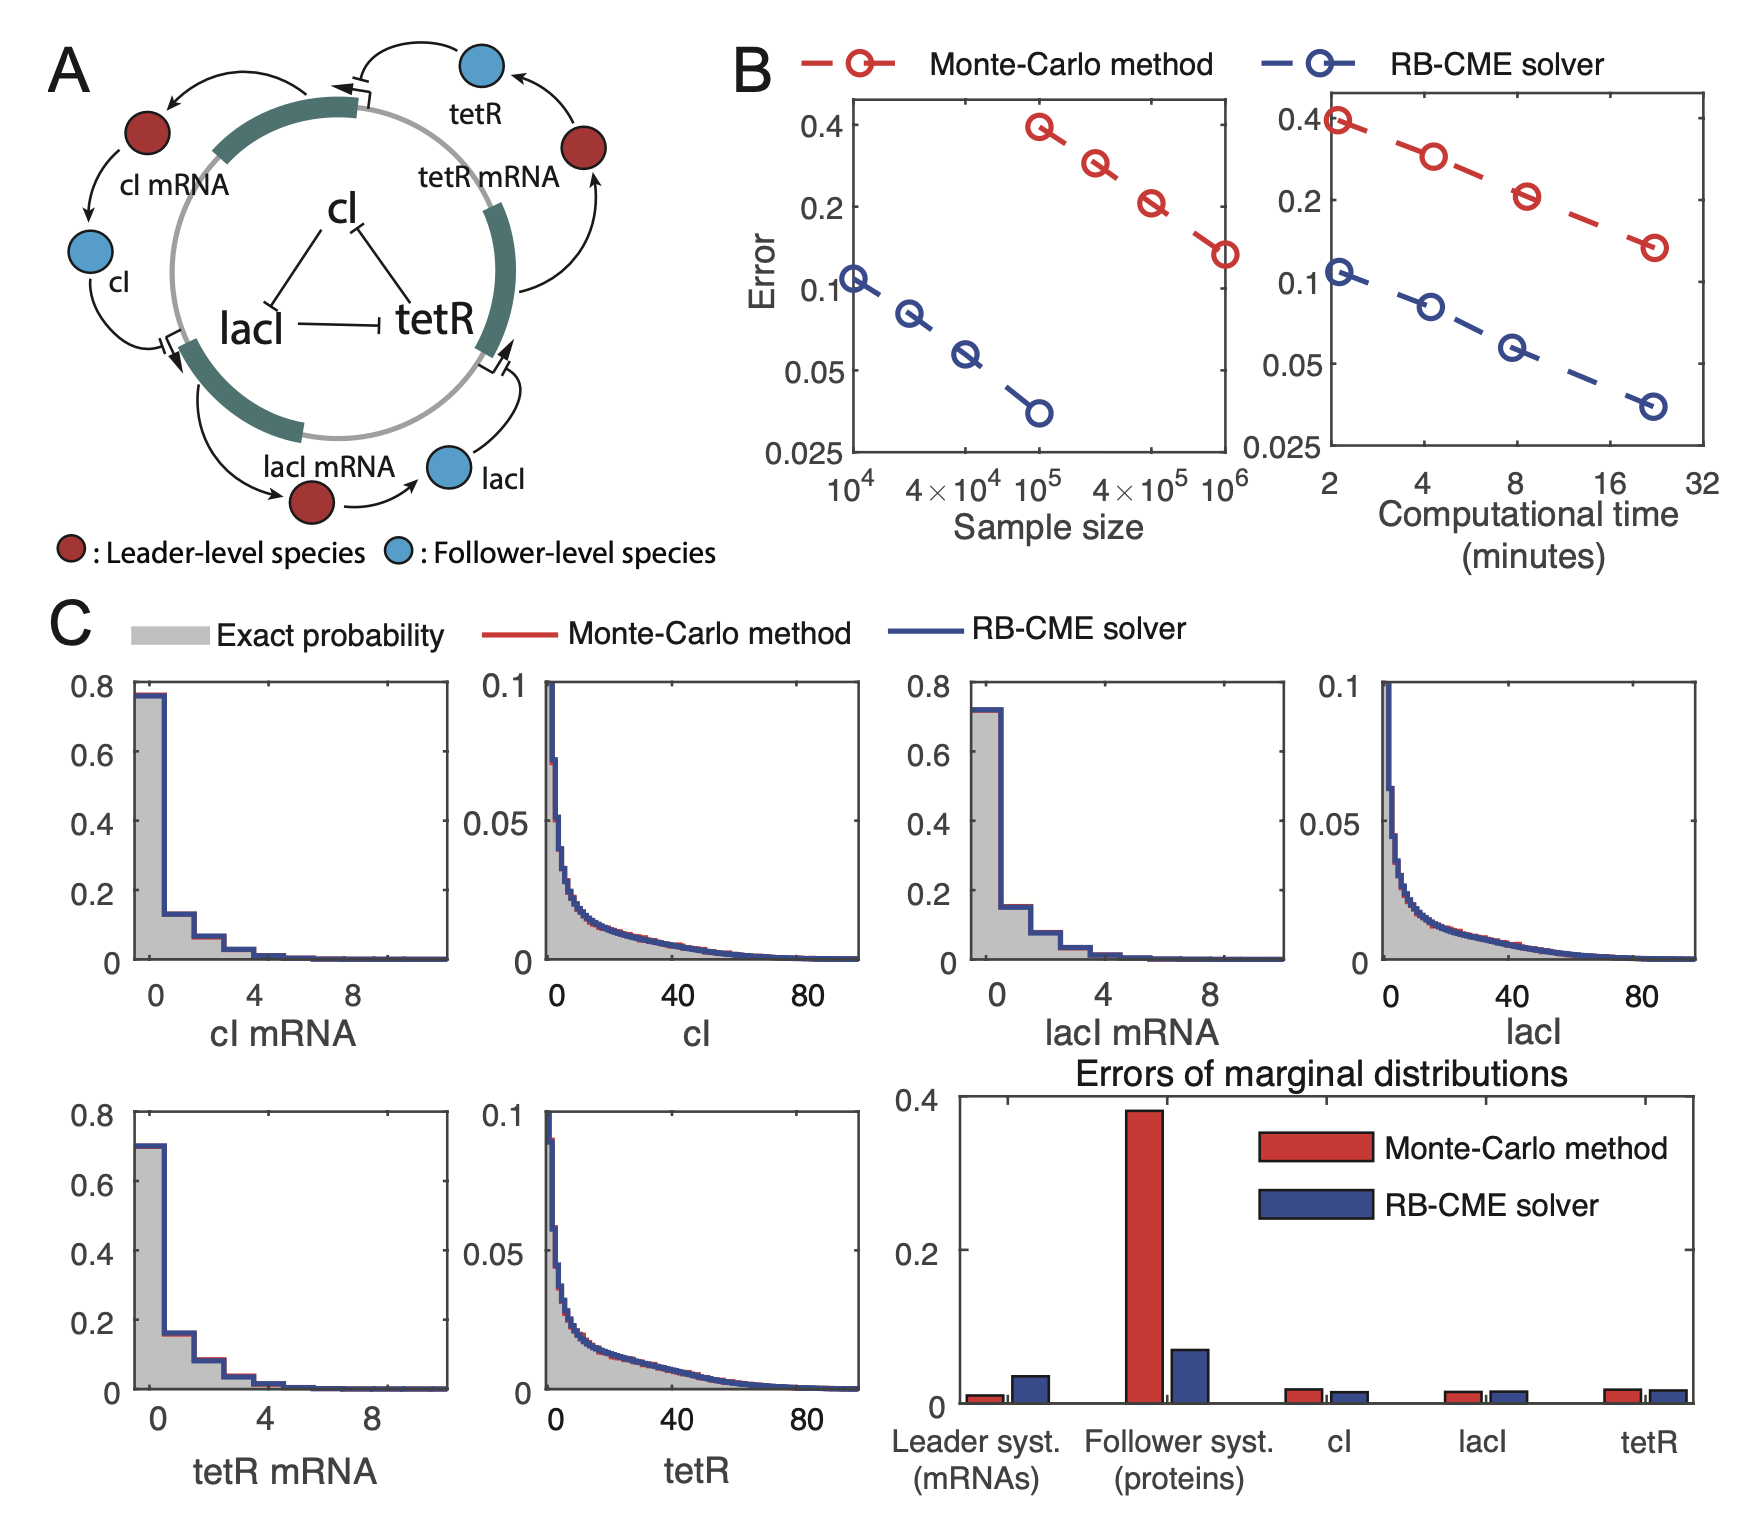
\includegraphics[width=6in]{isr/figs/represillator.png}
\caption{Performance of the RB-CME solver in the repressilator. (A) Diagram of the
repressilator with three gene expression systems whose proteins cyclically repress
each other. Our method classifies all the mRNAs as leader-level species and all the
proteins as follower-level species. (B) Convergence of the Monte-Carlo method and
the RB-CME solver (with the filtered FSP as the chosen filtering approach). We depict
the error by the sum of the L1 errors in estimating the leader system and the follower
system. The exact probability distribution is approximated by the Monte-Carlo method
with 3 × 10
9 samples.}
\end{center}
\end{figure}

\newpage

\section{Supplementary Information: Modeling of the Repressilator}
The repressilator model consists of three gene expression systems producing \( cI \), \( lacI \), and \( tetR \) respectively. The protein products cyclically repress each other’s expression. The chemical reactions are as follows:

\begin{align*}
    \emptyset \rightarrow{(\frac{\phi_1(t)}{1+X_6)^2)} + \phi_2} S_1 &\text{ Transcription}
    S_1  \xrightarrow{k_2} \emptyset &\text{ Degradation} \\
    
    S_1  \xrightarrow{k_3} S_1 + S_2 &\text{Translation} 
    S_2  \xrightarrow{k_4} \emptyset &\text{ Degradation} \\
    \emptyset  \xrightarrow{(1 + (\frac{{\phi_{1}}(t)}{\phi_2})^2)^{-1}} S_3 &\text{ (Transcription} 
    S_3  \xrightarrow{k_6} \emptyset &\text{ Degradation} \\
    S_3  \xrightarrow{k_7} S_3 + S_4 &\text{ Translation} 
    S_4  \xrightarrow{k_8} \emptyset &\text{ (Degradation)} \\
    \emptyset  \xrightarrow{(1 + (\frac{X_{\phi_{1}}(t)}{\phi_2})^2)^{-1}} S_5 &\text{ Transcription} 
    S_5  \xrightarrow{k_{10}} \emptyset &\text{ Degradation} \\
    S_5  \xrightarrow{k_{11}} S_5 + S_6 &\text{ Translation} 
    S_6  \xrightarrow{k_{12}} \emptyset &\text{Degradation}
\end{align*}

\begin{table}[h]
\centering
\begin{tabular}{@{}ll@{}}
\toprule
\textbf{Model parameter} & \textbf{Value} \\ 
\midrule
\( k_2 \) & 0.3 \( \min^{-1} \) \\
\( k_3 \) & 2 \( \min^{-1} \) \\
\( k_4 \) & 0.07 \( \min^{-1} \) \\
\( k_6 \) & 0.3 \( \min^{-1} \) \\
\( k_7 \) & 2 \( \min^{-1} \) \\
\( k_8 \) & 0.07 \( \min^{-1} \) \\
\( k_{10} \) & 0.3 \( \min^{-1} \) \\
\( k_{11} \) & 2 \( \min^{-1} \) \\
\( k_{12} \) & 0.07 \( \min^{-1} \) \\
\( \phi_1 \) & 0.5 \\
\( \phi_2 \) & \( 0.5 \times 10^{-4} \) \\
\midrule
\textbf{Initial condition} & \textbf{Value} \\ 
\midrule
\( X_1(0) \) & 1 \\
\( X_2(0) \) & 50 \\
\( X_3(0) \) & 0 \\
\( X_4(0) \) & 0 \\
\( X_5(0) \) & 0 \\
\( X_6(0) \) & 0 \\
\bottomrule
\end{tabular}
\caption{Model parameters and initial conditions for the repressilator model}
\end{table}







\newpage

\begin{algorithm}
\caption{Second-level decomposition for the RB-CME solver}
\begin{algorithmic}[1]
    \State Input the set of leader-level species and the set of follower-level species.
    \State Classify each follower-level species as an individual group. \Comment{Input}
    \For{$j = 1, \ldots, r$} \Comment{Initialization}
        \State Merge the groups that are involved in the $j$-th reaction. \Comment{Denote the merged group by $G_j$}
    \EndFor
    \For{$k = 1, \ldots, r_1$} \Comment{For $C_1$}
        \State Merge the groups that have species influencing $\lambda_k(x)$. \Comment{Denote the merged group by $G_k$}
        \For{$j = 1, \ldots, r$} \Comment{For $C_2$}
            \If{$j \in O_{\xi_k}$}
                \State Merge $\tilde{G}_k$ with the groups that have species influenced by the $j$-th reaction.
                \State $\tilde{G}_k \gets$ the group merged in the previous step.
            \EndIf
        \EndFor
    \EndFor
    \State Each group is a follower subsystem. \Comment{Output}
\end{algorithmic}
\end{algorithm}


\begin{algorithm}
\caption{Leader-follower decomposition for the RB-CME solver}
\begin{algorithmic}[1]
    \State Input the threshold $T$ for the maximum size of follower subsystems.
    \State Input a truncated state space $\{0,\ldots,TS_1 - 1\} \times \ldots \times \{0,\ldots,TS_n - 1\}$ that contains most probability $p(t,x)$. \Comment{Input}
    \State Largest\_size $\gets 0$. \Comment{Initialization}
    \State Figure out the $2^n$ choices of the first-level decomposition and give each an index.
    \For{$j = 1,\ldots,2^n$} \Comment{Search for the optimum}
        \State Use Algorithm 1 to obtain follower subsystems for the $j$-th first-level decomposition candidate.
        \State $l \gets$ the number of follower subsystems.
        \State Evaluate the size of each follower subsystem: $SS_i = \prod_{S'_i \in Z_i} Q'_{i}$.
        \If{$SS_i \leq T$ for all $i \in \{1,\ldots,l\}$ and $\prod_{i=1}^{l} SS_i >$ Largest\_size}
            \State Replace the optimal decomposition with the current one.
            \State Largest\_size $\gets \prod_{i=1}^{l} SS_i$.
        \EndIf
    \EndFor
    \State Output the optimal decomposition.
\end{algorithmic}
\end{algorithm}




\end{document}

